\documentclass[a4paper]{article}
%\usepackage{simplemargins}

%\usepackage[square]{natbib}
\usepackage{amsmath}
\usepackage{amsfonts}
\usepackage{amssymb}
\usepackage{graphicx}
\usepackage{subcaption}

\begin{document}
\pagenumbering{gobble}

\Large
 \begin{center}
     Opencast integration in Stud.IP\\

\hspace{10pt}

% Author names and affiliations
\large
Till Glöggler\\

\hspace{10pt}

\small
ELAN e.V.\\
Zentrum für Digitale Lehre, Campus Management
und Hochschuldidaktik\\
Universität Osnabrück\\
gloeggler@elan-ev.de\\


\end{center}

\hspace{10pt}

\normalsize
The LMS Stud.IP has had an Opencast integration provided by  a plugin for years. This plugin received
an complete overhaul recently, adding new features and an improved ui for users and admins.\\

New features include:
\begin{itemize}
    \item Working upload tool for files of nearly abritrary sizes,
    \item LTI integration for authentication and permission handling,
    \item Support for Opencast 3.x, 4.x and beyond
    \item Connection to multiple Opencast systems possible
    \item Comfortable configuration and maintenance
\end{itemize}

\begin{figure}[h!]
    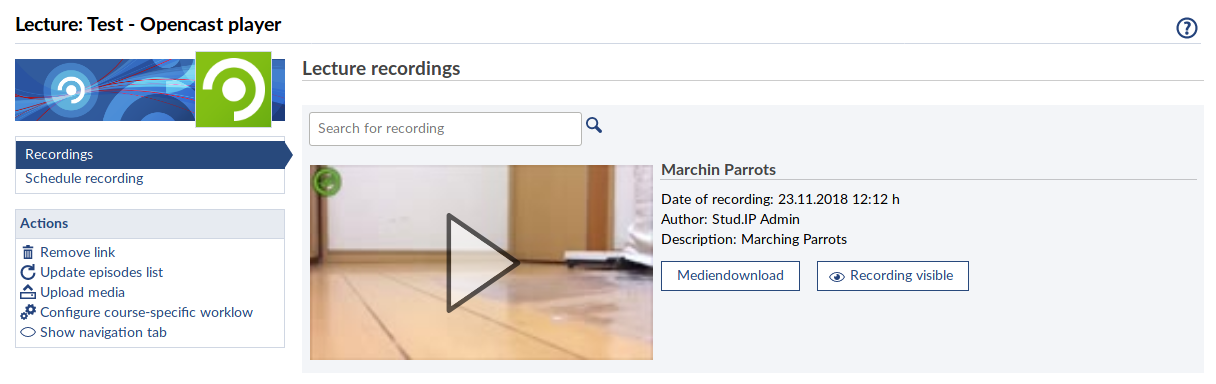
\includegraphics[width=\linewidth]{opencast-plugin-studip-user.png}
    \caption{Opencast user view.}

    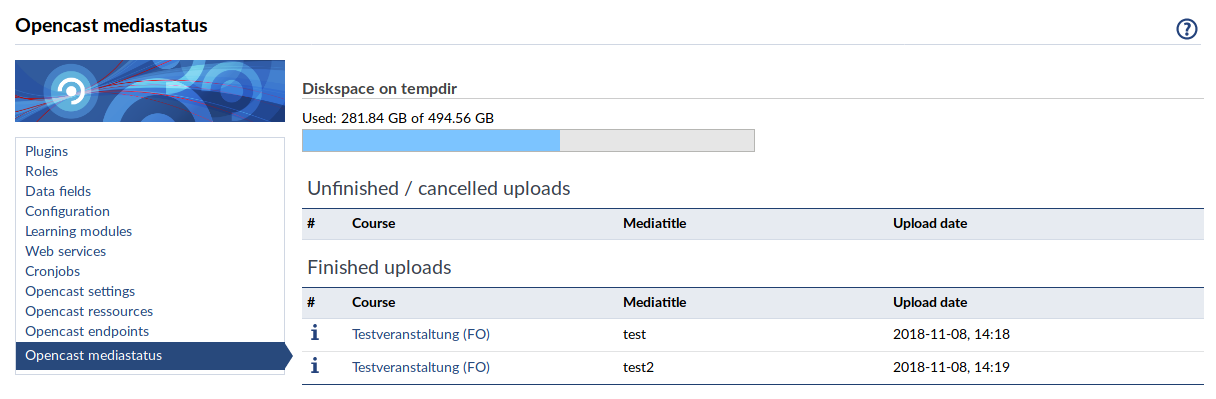
\includegraphics[width=\linewidth]{opencast-plugin-studip-admin.png}
    \caption{Opencast admin view.}
\end{figure}

\end{document}
